
\newcommand\instructionHeader[1]{{\large\tt \string#1}}

\chapter{RV32 Machine Instructions}
\label{chapter:RV32}
\index{RV32}

\section{Conventions and Terminology}

When discussing instructions, the following abbreviations/notations are used:

\subsection{XLEN}
\label{XLEN}

XLEN represents the bit-length of an \reg{x} register in the machine architecture.
Possible values are 32, 64 and 128.

\subsection{sx(val)}
\label{extension:sx}

Sign extend {\em val} to the left.

This is used to convert a signed integer value expressed using some number of
bits to a larger number of bits by adding more bits to the left.  In doing so,
the sign will be preserved.  In this case {\em val} represents the least
\acrshort{msb}s of the value.

For more on sign-extension see \autoref{SignExtension}.

\subsection{zx(val)}
\label{extension:zx}

Zero extend {\em val} to the left.

This is used to convert an unsigned integer value expressed using some number of
bits to a larger number of bits by adding more bits to the left.  In doing so,
the new bits added will all be set to zero.  As is the case with \verb@sx(val)@,
{\em val} represents the \acrshort{lsb}s of the final value.

For more on zero-extension see \autoref{ZeroExtension}.

\subsection{zr(val)}
\label{extension:zr}

Zero extend {\em val} to the right.

Some times a binary value is encoded such that a set of bits represented
by {\em val} are used to represent the \acrshort{msb}s of some longer (more bits)
value.
In this case it is necessary to append zeros to the right to convert \verb@val@ to
the longer value.

\autoref{Figure:ZeroRightExtend} illustrates converting a 20-bit {\em val} to
a 32-bit fullword.

\begin{figure}[ht]
  \centering
  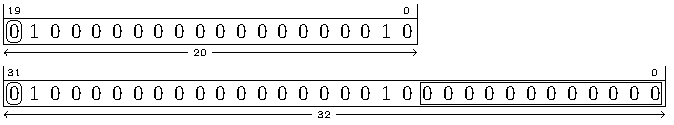
\includegraphics{figures/chapter05/ZeroRightExtend.pdf}
  \captionof{figure}{Zero-extending an integer to the right from 20 bits to 32 bits.}
  \label{Figure:ZeroRightExtend}
\end{figure}

%\begin{figure}[ht]
%\centering
%\parbox{.7\linewidth}{
%\DrawBitBoxUnsignedPicture{01000000000000000010}\\
%\DrawBitBoxUnsignedPicture{01000000000000000010000000000000}
%}
%\captionof{figure}{Zero-extending an integer to the right from 20 bits to 32 bits.}
%\label{Figure:ZeroRightExtend}
%\end{figure}


\subsection{Sign Extended Left and Zero Extend Right}
\label{extension:slzr}

Some instructions such as the J-type (see \autoref{insnformat:jtype}) include
immediate operands that are extended in both directions.

\autoref{Figure:slzrPositive} and \autoref{Figure:slzrNegative}
illustrates zero-extending a 20-bit negative number one bit to the right
and sign-extending it 11 bits to the left:

\begin{figure}[ht]
  \centering
  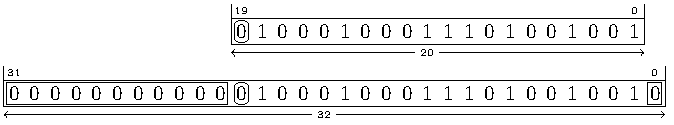
\includegraphics{figures/chapter05/slzrPositive.pdf}
  \captionof{figure}{Sign-extending a positive 20-bit number
  11 bits to the left and one bit to the right.}
  \label{Figure:slzrPositive}
\end{figure}

\begin{figure}[ht]
  \centering
  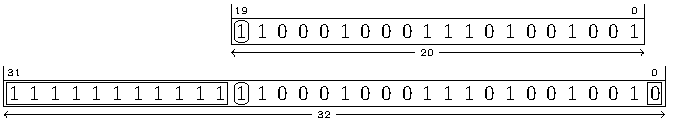
\includegraphics{figures/chapter05/slzrNegative.pdf}
  \captionof{figure}{Sign-extending a negative 20-bit number
  11 bits to the left and one bit to the right.}
  \label{Figure:slzrNegative}
\end{figure}

\subsection{m8(addr)}
\label{memory:m8}

The contents of an 8-bit value in memory at address {\em addr}.

Given the contents of the memory dump shown in
\autoref{Figure:SampleMemoryContents},
\verb@m8(0x42)@ refers to the memory location at address \verb@42@$_{16}$
that currently contains the 8-bit value \verb@fc@$_{16}$.

The \verb@m@$_n$\verb@(addr)@ notation can be used to refer to memory that is being
read or written depending on the context.

When memory is being written, the following notation is used to indicate that
the least significant 8 bis of {\em source} will be is written into memory at
the address {\em addr}:

\verb@m8(addr)@ $\leftarrow$ \verb@source@

When memory is being read, the following notation is used to indicate that the
8 bit value at the address {\em addr} will be read and stored into {\em dest}:

\verb@dest@ $\leftarrow$ \verb@m8(addr)@

Note that {\em source} and {\em dest} are typically registers.

\begin{figure}[ht]
\centering
\begin{BVerbatim}


00000030  2f 20 72 65 61 64 20 61  20 62 69 6e 61 72 79 20
00000040  66 69 fc 65 20 66 69 6c  6c 65 64 20 77 69 74 68
00000050  20 72 76 33 32 49 20 69  6e 73 74 72 75 63 74 69
00000060  6f 6e 73 20 61 6e 64 20  66 65 65 64 20 74 68 65
\end{BVerbatim}
\captionof{figure}{Sample memory contents.}
\label{Figure:SampleMemoryContents}
\end{figure}

\subsection{m16(addr)}
\label{memory:m16}

The contents of an 16-bit little-endian value in memory at address {\em addr}.

Given the contents of the memory dump shown in
\autoref{Figure:SampleMemoryContents},
\verb@m16(0x42)@ refers to the memory location at address \verb@42@$_{16}$
that currently contains \verb@65fc@$_{16}$. See also~\autoref{memory:m8}.

\subsection{m32(addr)}
\label{memory:m32}

The contents of an 32-bit little-endian value in memory at address {\em addr}.

Given the contents of the memory dump shown in
\autoref{Figure:SampleMemoryContents},
\verb@m32(0x42)@ refers to the memory location at address \verb@42@$_{16}$
that currently contains \verb@662065fc@$_{16}$.
See also~\autoref{memory:m8}.

\subsection{m64(addr)}

The contents of an 64-bit little-endian value in memory at address {\em addr}.

Given the contents of the memory dump shown in
\autoref{Figure:SampleMemoryContents},
\verb@m64(0x42)@ refers to the memory location at address \verb@42@$_{16}$
that currently contains \verb@656c6c69662065fc@$_{16}$.
See also~\autoref{memory:m8}.

\subsection{m128(addr)}

The contents of an 128-bit little-endian value in memory at
address {\em addr}.

Given the contents of the memory dump shown in
\autoref{Figure:SampleMemoryContents},
\verb@m128(0x42)@ refers to the memory location at address \verb@42@$_{16}$
that currently contains \verb@7220687469772064656c6c69662065fc@$_{16}$.
See also~\autoref{memory:m8}.

\subsection{.+offset}

The address of the current instruction plus a numeric offset.

\subsection{.-offset}

The address of the current instruction minus a numeric offset.

\subsection{pcrel\_13}
\label{pcrel.13}

An address that is within $[-4096..4094]$ $[$\verb@-0x1000..0x0ffe@$]$ of the current instruction location.
These addresses are typically expressed in assembly source code by using labels.
See \autoref{insnformat:btype} for examples.

\subsection{pcrel\_21}
\label{pcrel.21}

An address that is within $[-1048576..1048574]$ $[$\verb@-0x100000..0x0ffffe@$]$ of the current instruction
location.
These addresses are typically expressed in assembly source code by using labels.
See \autoref{insnformat:jtype} for an example.

\subsection{pc}

The current value of the program counter.

\subsection{rd}

An x-register used to store the result of instruction.

\subsection{rs1}

An x-register value used as a source operand for an instruction.

\subsection{rs2}

An x-register value used as a source operand for an instruction.

\subsection{imm}

An immediate numeric operand.  The word {\em immediate} refers
to the fact that the operand is stored within an instruction.

\subsection{rsN[h:l]}

The value of bits from {\em h} through {\em l} of x-register rsN.
For example: rs1[15:0] refers to the contents of
the 16 \acrshort{lsb}s of rs1.

\section{Addressing Modes}

immediate, register, base-displacement, pc-relative
\ednote{Write this section.}


\section{Instruction Encoding Formats}
\label{section:EncodingFormats}


%XXX Show and discuss a stack of formats explaining how the unnatural ordering
%of the {\em imm} fields reduces the number of possible locations that
%the hardware has to be prepared to {\em look} for various bits.  For example,
%the opcode, rd, rs1, rs1, func3 and the sign bit (when used) are all always
%in the same position.  Also note that imm[19:12] and imm[10:5] can only be
%found in one place.  imm[4:0] can only be found in one of two places\ldots

This document concerns itself with the RISC-V instruction formats shown
in \autoref{Figure:riscvFormats}.

%\autoref{Figure:riscvFormats} Shows the RISC-V instruction formats.

\begin{figure}[ht]
  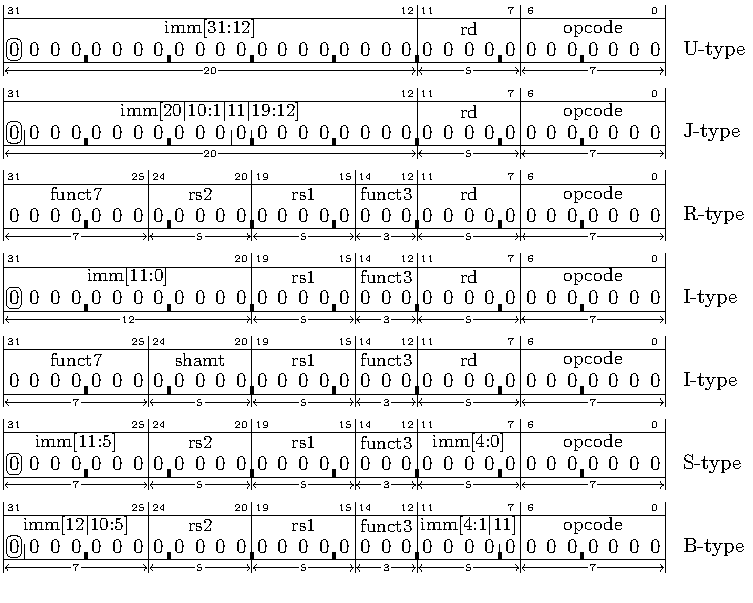
\includegraphics{figures/chapter05/riscvFormats.pdf}
  \captionof{figure}{RISC-V instruction formats.}
\label{Figure:riscvFormats}
\end{figure}

The method/format of the instructions has been designed with an eye on
the ease of future manufacture of the machine that will execute them.  It is
easier to build a machine if it does not have to accommodate many different
ways to perform the same task.  The result is that a machine can be
built with fewer gates, consumes less power, and can run faster than
if it were built when a priority is on how a user might prefer to decode
the same instructions from a hex dump.

Observe that all instructions have their opcode in bits 0-6 and when they
include an \verb@rd@ register it will be specified in bits 7-11,
an \verb@rs1@ register in bits 15-19, an \verb@rs2@ register in bits 20-24,
and so on.  This has a seemingly strange impact on the placement of any
immediate operands.

When immediate operands are present in an instruction, they are placed in
the remaining unused bits.  However, they are organized such that
the sign bit is {\em always} in bit 31 and the remaining bits placed so
as to minimize the number of places any given bit is located in different
instructions.

For example, consider immediate operand bits 12-19.  In the U-type format
they are in bit positions 12-19.  In the J-type format they are also in positions
12-19.  In the J-type format immediate operand bits 1-10 are in the same
instruction bit positions as they are in the I-type format and immediate
operand bits 5-10 are in the same positions as they are in the B-type and
S-type formats.

While this is inconvenient for anyone looking at a memory hexdump, it does
make sense when considering the impact of this choice on the number of
gates needed to implement circuitry to extract the immediate operands.

\subsection{U Type}
\label{insnformat:utype}

The U-Type format is used for instructions that use a 20-bit immediate operand
and an \verb@rd@ destination register.

%\DrawInsnTypeUTikz{11010110000000000011001010110111}

The \reg{rd} field contains an \reg{x} register number to be set to a value that
depends on the instruction.

%The imm field
%contains a 20-bit value that will be converted into \Gls{xlen} bits by
%using the {\em imm} operand for bits 31:12 and then sign-extending it
%to the left\footnote{When XLEN is larger than 32.} and zero-extending
%the LSBs as discussed in \autoref{extension:zr}.

If \Gls{xlen}=32 then the {\em imm} value will extracted from the instruction
and converted as shown in \autoref{Figure:u_type_decode} to form the
\verb@imm_u@ value.

\begin{figure}[ht]
  \centering
  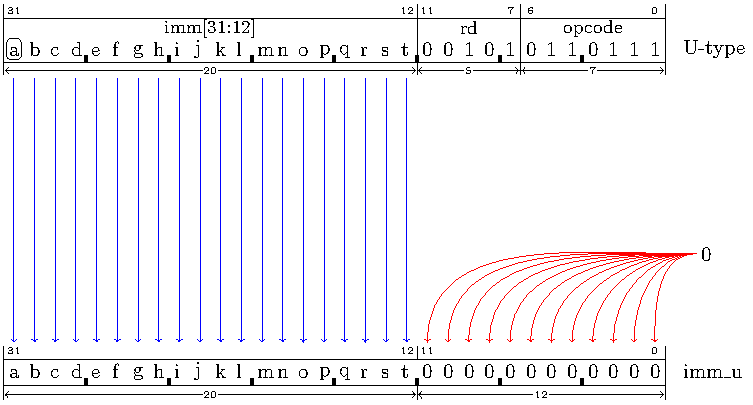
\includegraphics{figures/chapter05/UTypeDecode.pdf}
  \captionof{figure}{Decoding a U-type instruction.}
  \label{Figure:u_type_decode}
  \label{imm.u:decode}
  \index{imm\protect\_u}
\end{figure}

Notice that the 20-bits of the imm field are mapped in the same order and
in the same relative position that they appear in the instruction when
they are used to create the value of the immediate operand.
Leaving the imm bits on the left, in the ``upper bits'' of the \verb@imm_u@
value suggests a rationale for the name of this format.

\begin{itemize}
\item\instructionHeader{lui\ \ \ rd,imm}
\label{insn:lui}

Set register \verb@rd@ to the \verb@imm_u@ value as shown in \autoref{Figure:u_type_decode}.

For example: \verb@lui x23,0x12345@ will result in setting register \verb@x23@ to
the value \verb@0x12345000@.

\item\instructionHeader{auipc rd,imm}
\label{insn:auipc}

Add the address of the instruction to the \verb@imm_u@ value as
shown \autoref{Figure:u_type_decode} and store the result in register \verb@rd@.

For example, if the instruction \verb@auipc x22,0x10001@ is executed from
memory address \verb@0x800012f4@ then register \verb@x22@ will be set to
\verb@0x900022f4@.
\end{itemize}


If \Gls{xlen}=64 then the \verb@imm_u@ value in this example will be converted
to the same two's complement integer value by extending the sign-bit
further to the left.

\subsection{J Type}
\label{insnformat:jtype}

The J-type instruction format is used to encode the \verb@jal@ instruction
with an immediate value that determines the jump target address.
It is similar to the U-type, but the bits in the immediate operand are
arranged in a different order.

%\DrawInsnTypeJTikz{00111001001110000001001111101111}

Note that the \verb@imm_j@ value is
%expressed in the instruction as a target address that is converted to
an even 21-bit value in the range of
$[-1048576..1048574]$ $[$\verb@-0x100000..0x0ffffe@$]$ representing a \verb@pc@-relative offset to the
target address.

%In the J-type format the 20 {\em imm} bits are arranged such
%that they represent the ``lower'' portion of the immediate value.  Unlike
%the U-type instructions, the J-type requires the bits to be re-ordered
%and shifted to the right before they are used.
%\footnote{The reason that the J-type
%bits are reordered like this is because it simplifies the implementation of
%hardware as discussed in \autoref{section:EncodingFormats}.}

%The example above shows that the bit positions in the {\em imm} field
%description.  We see that the 20 {\em imm} bits are re-ordered according to:
%[20\textbar10:1\textbar11\textbar19:12].
%This means that the \acrshort{msb} of the {\em imm} field is to be placed
%into bit 20 of the immediate integer value ultimately used by the instruction
%when it is converted into \Gls{xlen} bits.
%The next bit to the right in the {\em imm} field is to be placed into bit 10 of
%the immediate value and so on.

%After the {\em imm} bits are re-positioned into bits 20:1 of the immediate value
%being constructed, a zero-bit will be added to the \acrshort{lsb}
%and the value in bit-position 20 will be replicated to sign-extend the
%value to \Gls{xlen} bits as discussed in \autoref{extension:slzr}.

If \Gls{xlen}=32 then the {\em imm} value will extracted from the
instruction and converted as shown in \autoref{Figure:j_type_decode} to
form the \verb@imm_j@ value.

\begin{figure}[ht]
  \centering
  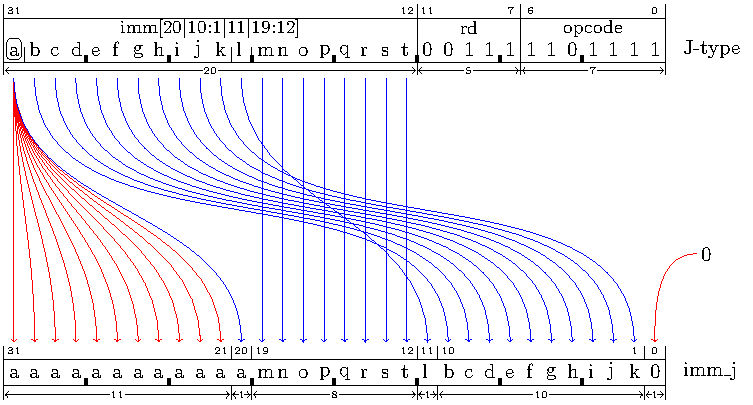
\includegraphics{figures/chapter05/JTypeDecode.pdf}
  \captionof{figure}{Decoding a J-type instruction.}
  \label{Figure:j_type_decode}
  \label{imm.j:decode}
  \index{imm\protect\_j}
\end{figure}


%\DrawBitBoxSignLeftZeroRightExtendedPicture{32}{01000000110111001001}{1}
%
%A J-type example with a negative imm field:
%
%\DrawInsnTypeJTikz{10111001001110000001001111101111}
%
%If \Gls{xlen}=32 then the {\em imm} field in this example will be converted as
%shown below.
%
%\DrawBitBoxSignLeftZeroRightExtendedPicture{32}{11000000110111001001}{1}

The J-type format is used by the Jump And Link instruction that calculates
the target address by adding \verb@imm_j@ to the current program
counter.  Since no instruction can be placed at an odd address the 20-bit
imm value is zero-extended to the right to represent a 21-bit signed offset
capable of expressing a wider range of target addresses than the 20-bit
imm value alone.

\begin{itemize}
\item\instructionHeader{jal\ \ \ rd,pcrel\_21}
\label{insn:jal}

Set register \verb@rd@ to the address of the next instruction that would
otherwise be executed (the address of the \verb@jal@ instruction + 4) and then
jump to the address given by the sum of the \verb@pc@ register and the
\verb@imm_j@ value as decoded from the instruction shown in
\autoref{imm.j:decode}.

Note that \verb@pcrel_21@ is expressed in the instruction as a target address
or label that is converted to a 21-bit value representing a \verb@pc@-relative
offset to the target address.
For example, consider the \verb@jal@ instructions in the following code:

\begin{verbatim}
00000010: 000002ef  jal    x5,0x10      # jump to self (address 0x10)
00000014: 008002ef  jal    x5,0x1c      # jump to address 0x1c
00000018: 00100073  ebreak
0000001c: 00100073  ebreak
\end{verbatim}

The instruction at address \verb@0x10@ has a target address of \verb@0x10@
and the \verb@imm_j@ is zero because offset from the ``current instruction''
to the target is zero.

The instruction at address \verb@0x14@ has a target address of \verb@0x1c@
and the \verb@imm_j@ is \verb@0x08@ because \verb@0x1c - 0x14 = 0x08@.

See also \autoref{insnformat:btype}.

\end{itemize}

\subsection{R Type}
\label{insnformat:rtype}

\begin{figure}[H]
  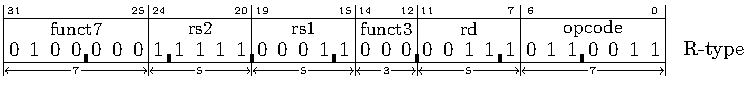
\includegraphics{figures/chapter05/RType.pdf}
\end{figure}


The R-type instructions are used for operations that set a destination
register \verb@rd@ to the result of an arithmetic, logical or shift operation
applied to source registers \verb@rs1@ and \verb@rs2@.

Note that instruction bit 30 (part of the the \verb@funct7@ field)
is used to select between the \verb@add@ and \verb@sub@ instructions
as well as to select between \verb@srl@ and \verb@sra@.

\begin{itemize}
\item\instructionHeader{add\ \ \ rd,rs1,rs2}
\label{insn:add}

Set register \verb@rd@ to \verb@rs1 + rs2@.

Note that the value of \verb@funct7@ must be zero for this instruction.
(The value of \verb@funct7@ is how the \verb@add@ instruction is differentiated
from the \verb@sub@ instruction.)

\item\instructionHeader{and\ \ \ rd,rs1,rs2}
\label{insn:and}

Set register \verb@rd@ to the bitwise \verb@and@ of \verb@rs1@ and  \verb@rs2@.

For example, if \verb@x17@ = \verb@0x55551111@ and \verb@x18@ = \verb@0xff00ff00@
then the instruction \verb@and x12,x17,x18@ will set \verb@x12@ to the
value \verb@0x55001100@.

\item\instructionHeader{or\ \ \ \ rd,rs1,rs2}
\label{insn:or}

Set register \verb@rd@ to the bitwise \verb@or@ of \verb@rs1@ and  \verb@rs2@.

For example, if \verb@x17@ = \verb@0x55551111@ and \verb@x18@ = \verb@0xff00ff00@
then the instruction \verb@or x12,x17,x18@ will set \verb@x12@ to the
value \verb@0xff55ff11@.

\item\instructionHeader{sll\ \ \ rd,rs1,rs2}
\label{insn:sll}

Shift \verb@rs1@ left by the number of bits specified in the least significant
5 bits of \verb@rs2@ and store the result in \verb@rd@.\footnote{\label{shift:xlen}
When XLEN is 64 or 128, the shift distance will be given by the least-significant
6 or 7 bits of \texttt{rs2} respectively.
For more information on how shifting works, see \autoref{shifting}.}

For example, if \verb@x17@ = \verb@0x12345678@ and \verb@x18@ = \verb@0x08@
then the instruction \verb@sll x12,x17,x18@ will set \verb@x12@ to the
value \verb@0x34567800@.

\item\instructionHeader{slt\ \ \ rd,rs1,rs2}
\label{insn:slt}

If the signed integer value in \verb@rs1@ is less than the
signed integer value in \verb@rs2@ then set \verb@rd@ to \verb@1@.
Otherwise, set \verb@rd@ to \verb@0@.

For example, if \verb@x17@ = \verb@0x12345678@ and \verb@x18@ = \verb@0x0000ffff@
then the instruction \verb@slt x12,x17,x18@ will set \verb@x12@ to the
value \verb@0x00000000@.

If \verb@x17@ = \verb@0x82345678@ and \verb@x18@ = \verb@0x0000ffff@
then the instruction \verb@slt x12,x17,x18@ will set \verb@x12@ to the
value \verb@0x00000001@.

\item\instructionHeader{sltu\ \ rd,rs1,rs2}
\label{insn:sltu}

If the unsigned integer value in \verb@rs1@ is less than the
unsigned integer value in \verb@rs2@ then set \verb@rd@ to \verb@1@.
Otherwise, set \verb@rd@ to \verb@0@.

For example, if \verb@x17@ = \verb@0x12345678@ and \verb@x18@ = \verb@0x0000ffff@
then the instruction \verb@sltu x12,x17,x18@ will set \verb@x12@ to the
value \verb@0x00000000@.

If \verb@x17@ = \verb@0x12345678@ and \verb@x18@ = \verb@0x8000ffff@
then the instruction \verb@sltu x12,x17,x18@ will set \verb@x12@ to the
value \verb@0x00000001@.

\item\instructionHeader{sra\ \ \ rd,rs1,rs2}
\label{insn:sra}

Arithmetic-shift \verb@rs1@ right by the number of bits given in the least-significant
5 bits of the \verb@rs2@ register and store the result in
\verb@rd@.\footref{shift:xlen}

For example, if \verb@x17@ = \verb@0x87654321@ and \verb@x18@ = \verb@0x08@
then the instruction \verb@sra x12,x17,x18@ will set \verb@x12@ to the
value \verb@0xff876543@.

If \verb@x17@ = \verb@0x76543210@ and \verb@x18@ = \verb@0x08@
then the instruction \verb@sra x12,x17,x18@ will set \verb@x12@ to the
value \verb@0x00765432@.

Note that the value of \verb@funct7@ must be zero for this instruction.
(The value of \verb@funct7@ is how the \verb@sra@ instruction is differentiated
from the \verb@srl@ instruction.)

\item\instructionHeader{srl\ \ \ rd,rs1,rs2}
\label{insn:srl}

Logic-shift \verb@rs1@ right by the number of bits given in the least-significant
5 bits of the \verb@rs2@ register and store the result in
\verb@rd@.\footref{shift:xlen}

For example, if \verb@x17@ = \verb@0x87654321@ and \verb@x18@ = \verb@0x08@
then the instruction \verb@srl x12,x17,x18@ will set \verb@x12@ to the
value \verb@0x00876543@.

If \verb@x17@ = \verb@0x76543210@ and \verb@x18@ = \verb@0x08@
then the instruction \verb@srl x12,x17,x18@ will set \verb@x12@ to the
value \verb@0x00765432@.

Note that the value of \verb@funct7@ must be \verb@0b0100000@ for this instruction.
(The value of \verb@funct7@ is how the \verb@srl@ instruction is differentiated
from the \verb@sra@ instruction.)

\item\instructionHeader{sub\ \ \ rd,rs1,rs2}
\label{insn:sub}

Set register \verb@rd@ to \verb@rs1 - rs2@.

Note that the value of \verb@funct7@ must be \verb@0b0100000@ for this instruction.
(The value of \verb@funct7@ is how the \verb@sub@ instruction is differentiated
from the \verb@add@ instruction.)

\item\instructionHeader{xor\ \ \ rd,rs1,rs2}
\label{insn:xor}

Set register \verb@rd@ to the bitwise \verb@xor@ of \verb@rs1@ and  \verb@rs2@.

For example, if \verb@x17@ = \verb@0x55551111@ and \verb@x18@ = \verb@0xff00ff00@
then the instruction \verb@xor x12,x17,x18@ will set \verb@x12@ to the
value \verb@0xaa55ee11@.

\end{itemize}

\subsection{I Type}
\label{insnformat:itype}
%\DrawInsnTypeITikz{00000000010000011000001110000011}

The I-type instruction format is used to encode instructions with a
signed 12-bit immediate operand with a range of $[-2048..2047]$,
an \verb@rd@ register, and an \verb@rs1@ register.

If \Gls{xlen}=32 then the 12-bit {\em imm} value example will extracted from
the instruction and converted as shown in \autoref{Figure:i_type_decode}
to form the \verb@imm_i@ value.

\begin{figure}[ht]
  \centering
  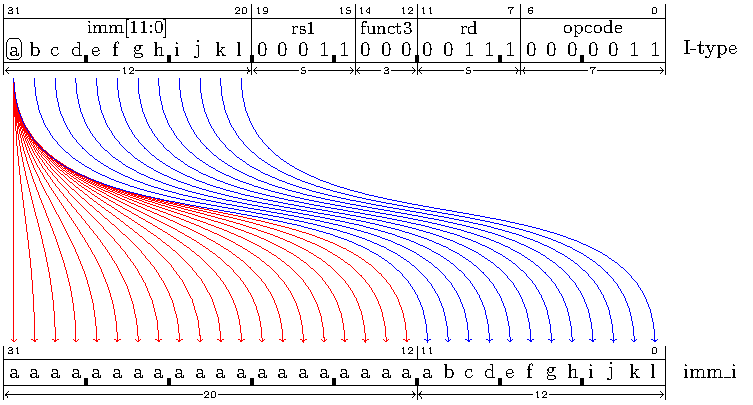
\includegraphics{figures/chapter05/ITypeDecode.pdf}
  \captionof{figure}{Decoding an I-type Instruction.}
  \label{Figure:i_type_decode}
  \label{imm.i:decode}
  \index{imm\protect\_i}
\end{figure}

A special case of the I-type is used for shift-immediate instructions
where the imm field is used to represent the number of bit positions
to shift as shown in \autoref{Figure:shamt_i_type_decode}.
In this variation, the least significant five bits of the imm field are
extracted to form the \verb@shamt_i@
value.\footnote{When XLEN is 64 or 128, the \texttt{shamt\_i} field will
consist of 6 or 7 bits respectively.}

Note also that bit 30 (the imm instruction field bit labeled `\verb@b@') is used to select
between arithmetic and logical shifting.

\begin{figure}[ht]
  \centering
  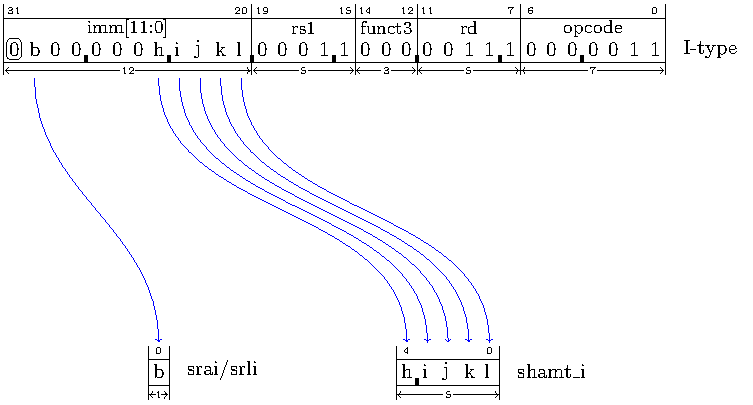
\includegraphics{figures/chapter05/ITypeShiftDecode.pdf}
  \captionof{figure}{Decoding an I-type Shift Instruction.}
  \label{Figure:shamt_i_type_decode}
  \label{shamt.i:decode}
  \index{shamt\protect\_i}
\end{figure}


\begin{figure}[ht]
\centering
\begin{verbatim}
 00002640: 6f 00 00 00 6f 00 00 00  b7 87 00 00 03 a5 07 43 *o...o..........C*
 00002650: 67 80 00 00 00 00 00 00  76 61 6c 3d 00 00 00 00 *g.......val=....*
 00002660: 00 00 00 00 80 84 2e 41  1f 85 45 41 80 40 9a 44 *.......A..EA.@.D*
 00002670: 4f 11 f3 c3 6e 8a 67 41  20 1b 00 00 20 1b 00 00 *O...n.gA ... ...*
 00002680: 44 1b 00 00 14 1b 00 00  14 1b 00 00 04 1c 00 00 *D...............*
\end{verbatim}
\captionof{figure}{An Example Memory Dump.}
\label{Figure:imm:memory:dump}
\end{figure}


\begin{itemize}
\item\instructionHeader{addi\ \ rd,rs1,imm}
\label{insn:addi}

Set register \verb@rd@ to \verb@rs1 + imm_i@.

\item\instructionHeader{andi\ \ rd,rs1,imm}
\label{insn:andi}

Set register \verb@rd@ to the bitwise \verb@and@ of \verb@rs1@ and \verb@imm_i@.

For example, if \verb@x17@ = \verb@0x55551111@ then the instruction
\verb@andi x12,x17,0x0ff@ will set \verb@x12@ to the value \verb@0x00000011@.

Recall that \verb@imm@ is sign-extended.
Therefore if \verb@x17@ = \verb@0x55551111@ then the instruction
\verb@andi x12,x17,0x800@ will set \verb@x12@ to the value \verb@0x55551000@.

\item\instructionHeader{jalr\ \ rd,imm(rs1)}
\label{insn:jalr}

Set register \verb@rd@ to the address of the next instruction that would
otherwise be executed (the address of the \verb@jalr@ instruction + 4) and then
jump to an address given by the sum of the \verb@rs1@ register and the
\verb@imm_i@ value as decoded from the instruction shown in \autoref{imm.i:decode}.

Note that the \verb@pc@ register can never refer to an odd address.
This instruction will explicitly set the \acrshort{lsb} to zero regardless
of the value of the value of the calculated target address.

\item\instructionHeader{lb\ \ \ \ rd,imm(rs1)}
\label{insn:lb}

Set register \verb@rd@ to the value of the sign-extended byte fetched from
the memory address given by the sum of \verb@rs1@ and \verb@imm_i@.

For example, given the memory contents shown in \autoref{Figure:imm:memory:dump},
if register \verb@x13@ = \verb@0x00002650@ then the instruction
\verb@lb x12,1(x13)@ will set \verb@x12@ to the value \verb@0xffffff80@.

\item\instructionHeader{lbu\ \ \ rd,imm(rs1)}
\label{insn:lbu}

Set register \verb@rd@ to the value of the zero-extended byte fetched from
the memory address given by the sum of \verb@rs1@ and \verb@imm_i@.

For example, given the memory contents shown in \autoref{Figure:imm:memory:dump},
if register \verb@x13@ = \verb@0x00002650@ then the instruction
\verb@lbu x12,1(x13)@ will set \verb@x12@ to the value \verb@0x00000080@.

\item\instructionHeader{lh\ \ \ \ rd,imm(rs1)}
\label{insn:lh}

Set register \verb@rd@ to the value of the sign-extended 16-bit little-endian
half-word value fetched from the memory address given by the sum
of \verb@rs1@ and \verb@imm_i@.

For example, given the memory contents shown in \autoref{Figure:imm:memory:dump},
if register \verb@x13@ = \verb@0x00002650@ then the instruction
\verb@lh x12,-2(x13)@ will set \verb@x12@ to the value \verb@0x00004307@.

If register \verb@x13@ = \verb@0x00002650@ then the instruction
\verb@lh x12,-8(x13)@ will set \verb@x12@ to the value \verb@0xffff87b7@.

\item\instructionHeader{lhu\ \ \ rd,imm(rs1)}
\label{insn:lhu}

Set register \verb@rd@ to the value of the zero-extended 16-bit little-endian
half-word value fetched from the memory address given by the sum
of \verb@rs1@ and \verb@imm_i@.

For example, given the memory contents shown in \autoref{Figure:imm:memory:dump},
if register \verb@x13@ = \verb@0x00002650@ then the instruction
\verb@lhu x12,-2(x13)@ will set \verb@x12@ to the value \verb@0x00004307@.

If register \verb@x13@ = \verb@0x00002650@ then the instruction
\verb@lhu x12,-8(x13)@ will set \verb@x12@ to the value \verb@0x000087b7@.

\item\instructionHeader{lw\ \ \ \ rd,imm(rs1)}
\label{insn:lw}

Set register \verb@rd@ to the value of the sign-extended 32-bit little-endian
word value fetched from the memory address given by the sum
of \verb@rs1@ and \verb@imm_i@.

For example, given the memory contents shown in \autoref{Figure:imm:memory:dump},
if register \verb@x13@ = \verb@0x00002650@ then the instruction
\verb@lw x12,-4(x13)@ will set \verb@x12@ to the value \verb@4307a503@.


\item\instructionHeader{ori\ \ \ rd,rs1,imm}
\label{insn:ori}

Set register \verb@rd@ to the bitwise \verb@or@ of \verb@rs1@ and \verb@imm_i@.

For example, if \verb@x17@ = \verb@0x55551111@ then the instruction
\verb@ori x12,x17,0x0ff@ will set \verb@x12@ to the value \verb@0x555511ff@.

Recall that \verb@imm@ is sign-extended.
Therefore if \verb@x17@ = \verb@0x55551111@ then the instruction
\verb@ori x12,x17,0x800@ will set \verb@x12@ to the value \verb@0xfffff911@.

\item\instructionHeader{slli\ \ rd,rs1,imm}
\label{insn:slli}

Shift \verb@rs1@ left by the number of bits specified in \verb@shamt_i@
(as shown in \autoref{shamt.i:decode})
and store the result in \verb@rd@.\footnote{\label{shifti:xlen}
When XLEN is 64 or 128, the shift distance will be given by the least-significant
6 or 7 bits of the imm field respectively.
For more information on how shifting works, see \autoref{shifting}.}

For example, if \verb@x17@ = \verb@0x12345678@ then the instruction
\verb@slli x12,x17,4@ will set \verb@x12@ to the value \verb@0x23456780@.

\item\instructionHeader{slti\ \ rd,rs1,imm}
\label{insn:slti}

If the signed integer value in \verb@rs1@ is less than the
signed integer value in \verb@imm_i@ then set \verb@rd@ to \verb@1@.
Otherwise, set \verb@rd@ to \verb@0@.

\item\instructionHeader{sltiu\ rd,rs1,imm}
\label{insn:sltiu}

If the unsigned integer value in \verb@rs1@ is less than the
unsigned integer value in \verb@imm_i@ then set \verb@rd@ to \verb@1@.
Otherwise, set \verb@rd@ to \verb@0@.

Note that \verb@imm_i@ is always created by sign-extending the \verb@imm@ value
as shown in \autoref{imm.i:decode} even though it is then later used as an unsigned
integer for the purposes of comparing its magnitude to the unsigned value in rs1.
Therefore, this instruction provides a method to compare \verb@rs1@ to a value
in the ranges of
$[\text{\tt 0}..\text{\tt 0x7ff}]$ and $[\text{\tt 0xfffff800}..\text{\tt 0xffffffff}]$.

\item\instructionHeader{srai\ \ rd,rs1,imm}
\label{insn:srai}

Arithmetic-shift \verb@rs1@ right by the number of bits specified in \verb@shamt_i@
(as shown in \autoref{shamt.i:decode})
and store the result in \verb@rd@.\footref{shifti:xlen}

For example, if \verb@x17@ = \verb@0x87654321@ then the instruction
\verb@srai x12,x17,4@ will set \verb@x12@ to the value \verb@0xf8765432@.

Note that the value of bit 30 must be 1 for this instruction.
(The value of bit 30 is how the \verb@srai@ instruction is differentiated
from the \verb@srli@ instruction.)

\item\instructionHeader{srli\ \ rd,rs1,imm}
\label{insn:srli}

Logic-shift \verb@rs1@ right by the number of bits specified in \verb@shamt_i@
(as shown in \autoref{shamt.i:decode})
and store the result in \verb@rd@.\footref{shifti:xlen}

For example, if \verb@x17@ = \verb@0x87654321@ then the instruction
\verb@srli x12,x17,4@ will set \verb@x12@ to the value \verb@0x08765432@.

Note that the value of bit 30 must be 0 for this instruction.
(The value of bit 30 is how the \verb@srli@ instruction is differentiated
from the \verb@srai@ instruction.)

\item\instructionHeader{xori\ \ rd,rs1,imm}
\label{insn:xori}

Set register \verb@rd@ to the bitwise \verb@xor@ of \verb@rs1@ and \verb@imm_i@.

For example, if \verb@x17@ = \verb@0x55551111@ then the instruction
\verb@xori x12,x17,0x0ff@ will set \verb@x12@ to the value \verb@0x555511ee@.

Recall that \verb@imm@ is sign-extended.
Therefore if \verb@x17@ = \verb@0x55551111@ then
\verb@xori x12,x17,0x800@ will set \verb@x12@ to the value \verb@0xaaaae911@.

\end{itemize}

\subsection{S Type}
\label{insnformat:stype}
%\DrawInsnTypeSTikz{00000000111100011000100110100011}

The S-type instruction format is used to encode instructions with a
signed 12-bit immediate operand with a range of $[-2048..2047]$,
an \verb@rs1@ register, and an \verb@rs2@ register.

If \Gls{xlen}=32 then the 12-bit {\em imm} value example will extracted
from the instruction and converted as shown \autoref{Figure:imm_s_type_decode}
to form the \verb@imm_s@ value.

\begin{figure}[ht]
  \centering
  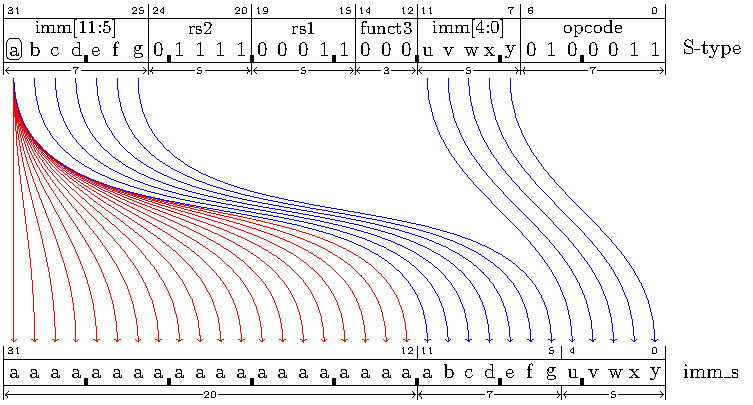
\includegraphics{figures/chapter05/STypeDecode.pdf}
  \captionof{figure}{Decoding an S-type Instruction.}
  \label{Figure:imm_s_type_decode}
  \label{imm.s:decode}
  \index{imm\protect\_s}
\end{figure}

\begin{itemize}
\item\instructionHeader{sb\ \ \ \ rs2,imm(rs1)}
\label{insn:sb}

Set the byte of memory at the address given by the sum of \verb@rs1@ and
\verb@imm_s@ to the 8 \acrshort{lsb}s of \verb@rs2@.

For example, given the memory contents shown in \autoref{Figure:imm:memory:dump},
if registers \verb@x13@ = \verb@0x00002650@ and \verb@x12@ = \verb@0x12345678@
then the instruction \verb@sb x12,1(x13)@ will change the memory byte at address
\verb@0x00002651@ from \verb@0x80@ to \verb@0x78@ resulting in:

\begin{verbatim}
 00002640: 6f 00 00 00 6f 00 00 00  b7 87 00 00 03 a5 07 43 *o...o..........C*
 00002650: 67 78 00 00 00 00 00 00  76 61 6c 3d 00 00 00 00 *gx......val=....*
 00002660: 00 00 00 00 80 84 2e 41  1f 85 45 41 80 40 9a 44 *.......A..EA.@.D*
 00002670: 4f 11 f3 c3 6e 8a 67 41  20 1b 00 00 20 1b 00 00 *O...n.gA ... ...*
 00002680: 44 1b 00 00 14 1b 00 00  14 1b 00 00 04 1c 00 00 *D...............*
\end{verbatim}

\item\instructionHeader{sh\ \ \ \ rs2,imm(rs1)}
\label{insn:sh}

Set the 16-bit half-word of memory at the address given by the sum of \verb@rs1@ and
\verb@imm_s@ to the 16 \acrshort{lsb}s of \verb@rs2@.

For example, given the memory contents shown in \autoref{Figure:imm:memory:dump},
if registers \verb@x13@ = \verb@0x00002650@ and \verb@x12@ = \verb@0x12345678@
then the instruction \verb@sh x12,2(x13)@ will change the memory half-word at
address \verb@0x00002652@ from \verb@0x0000@ to \verb@0x5678@ resulting in:

\begin{verbatim}
 00002640: 6f 00 00 00 6f 00 00 00  b7 87 00 00 03 a5 07 43 *o...o..........C*
 00002650: 67 80 78 56 00 00 00 00  76 61 6c 3d 00 00 00 00 *g.xV....val=....*
 00002660: 00 00 00 00 80 84 2e 41  1f 85 45 41 80 40 9a 44 *.......A..EA.@.D*
 00002670: 4f 11 f3 c3 6e 8a 67 41  20 1b 00 00 20 1b 00 00 *O...n.gA ... ...*
 00002680: 44 1b 00 00 14 1b 00 00  14 1b 00 00 04 1c 00 00 *D...............*
\end{verbatim}

\item\instructionHeader{sw\ \ \ \ rs2,imm(rs1)}
\label{insn:sw}

Store the 32-bit value in \verb@rs2@ into the memory at the address given
by the sum of \verb@rs1@ and \verb@imm_s@.

For example, given the memory contents shown in \autoref{Figure:imm:memory:dump},
if registers \verb@x13@ = \verb@0x00002650@ and \verb@x12@ = \verb@0x12345678@
then the instruction \verb@sw x12,0(x13)@ will change the memory word at address
\verb@0x00002650@ from \verb@0x00008067@ to \verb@0x12345678@ resulting in:

\begin{verbatim}
 00002640: 6f 00 00 00 6f 00 00 00  b7 87 00 00 03 a5 07 43 *o...o..........C*
 00002650: 78 56 34 12 00 00 00 00  76 61 6c 3d 00 00 00 00 *xV4.....val=....*
 00002660: 00 00 00 00 80 84 2e 41  1f 85 45 41 80 40 9a 44 *.......A..EA.@.D*
 00002670: 4f 11 f3 c3 6e 8a 67 41  20 1b 00 00 20 1b 00 00 *O...n.gA ... ...*
 00002680: 44 1b 00 00 14 1b 00 00  14 1b 00 00 04 1c 00 00 *D...............*
\end{verbatim}

\end{itemize}

%%%%%%%%%%%%%%%%%%%%%%%%%%%%%%%%%%%%%%%%%%%%%%%%%%%%%%%%%%%%%%%%%%%%%%%%%%%%%%%%
\subsection{B Type}
\label{insnformat:btype}
%\DrawInsnTypeBTikz{00000000111100011000100011100011}

The B-type instruction format is used for branch instructions that
require an even immediate value that is used to determine the
branch target address as an offset from the current instruction's
address.

If \Gls{xlen}=32 then the 12-bit {\em imm} value example will extracted from
the instruction and converted as shown in \autoref{Figure:imm_b_type_decode}
to form the \verb@imm_b@ value.

\begin{figure}[ht]
  \centering
  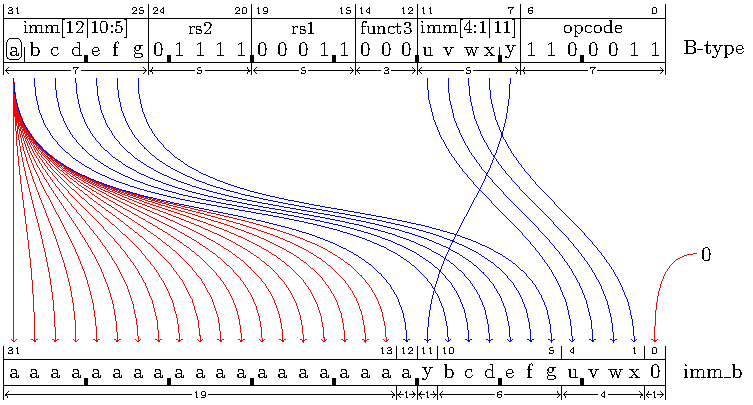
\includegraphics{figures/chapter05/BTypeDecode.pdf}
  \captionof{figure}{Decoding a B-type Instruction.}
  \label{Figure:imm_b_type_decode}
  \label{imm.b:decode}
  \index{imm\protect\_b}
\end{figure}

Note that \verb@imm_b@ is expressed in the instruction as a target
address that is converted to an even 13-bit value in the range of
$[-4096..4094]$ $[$\verb@-0x1000..0x0ffe@$]$ representing a \verb@pc@-relative offset to the
target address. For example, consider the branch instructions in
the following code:

\begin{verbatim}
00000000: 00520063  beq    x4,x5,0x0    # branches to self (address 0x0)
00000004: 00520463  beq    x4,x5,0xc    # branches to address 0xc
00000008: fe520ce3  beq    x4,x5,0x0    # branches to address 0x0
0000000c: 00100073  ebreak
\end{verbatim}

The instruction at address \verb@0x0@ has a target address of zero and
\verb@imm_b@ is zero because the offset from the ``current instruction''
to the target is zero.\footnote{This is in contrast to many other
instruction sets with \texttt{pc}-relative addressing modes that express
a branch target offset from the ``next instruction.''}

The instruction at address \verb@0x4@ has a target address of \verb@0xc@
and it has an \verb@imm_b@ of \verb@0x08@ because \verb@0x4 + 0x08 = 0x0c@.

The instruction at address \verb@0x8@ has a target address of zero and
\verb@imm_b@ is \verb@0xfffffff8@ (-8) because \verb@0x8 + 0xfffffff8 = 0x0@.

\begin{itemize}
\item\instructionHeader{beq\ \ \ rs1,rs2,pcrel\_13}
\label{insn:beq}

If \verb@rs1@ is equal to \verb@rs2@ then add \verb@imm_b@ to the
\verb@pc@ register.

\item\instructionHeader{bge\ \ \ rs1,rs2,pcrel\_13}
\label{insn:bge}

If the signed value in \verb@rs1@ is greater than or equal to the
signed value in \verb@rs2@ then add \verb@imm_b@ to the
\verb@pc@ register.

\item\instructionHeader{bgeu\ \ rs1,rs2,pcrel\_13}
\label{insn:bgeu}

If the unsigned value in \verb@rs1@ is greater than or equal to the
unsigned value in \verb@rs2@ then add \verb@imm_b@ to the
\verb@pc@ register.

\item\instructionHeader{blt\ \ \ rs1,rs2,pcrel\_13}
\label{insn:blt}

If the signed value in \verb@rs1@ is less than the
signed value in \verb@rs2@ then add \verb@imm_b@ to the
\verb@pc@ register.

\item\instructionHeader{bltu\ \ rs1,rs2,pcrel\_13}
\label{insn:bltu}

If the unsigned value in \verb@rs1@ is less than the
unsigned value in \verb@rs2@ then add \verb@imm_b@ to the
\verb@pc@ register.

\item\instructionHeader{bne\ \ \ rs1,rs2,pcrel\_13}
\label{insn:bne}

If \verb@rs1@ is not equal to \verb@rs2@ then add \verb@imm_b@ to the
\verb@pc@ register.

\end{itemize}

%\label{insn:bgt}
%\label{insn:ble}
%\label{insn:bgtu}
%\label{insn:beqz}
%\label{insn:bnez}
%\label{insn:blez}
%\label{insn:bgez}
%\label{insn:bltz}
%\label{insn:bgtz}


%Control and Status Register Instructions
%\label{insn:csrrw}
%\label{insn:csrrs}
%\label{insn:csrrc}
%\label{insn:csrrwi}
%\label{insn:csrrsi}
%\label{insn:csrrci}


\section{CPU Registers}
\label{cpuregs}

The registers are names x0 through x31 and have aliases suited to their
conventional use.  The following table describes each register.

Note
\ednote{Need to add a section that discusses the calling conventions}
that the calling calling convention specifies that only some
of the registers are to be saved by functions if they alter their contents.
The idea being that accessing memory is time-consuming and that by
classifying some registers as ``temporary'' (not saved by any function
that alter its contents) it is possible to carefully implement a function
with less need to store register values on the stack in order to use them
to perform the operations of the function.

The lack of grouping the temporary and saved registers is due to the
fact that the E extension %\cite{XXX}
only has the first 16 registers
and some of the instructions in the C extension %See \autoref{rv32:c}
can only refer to the first 16 registers.


\begin{center}
\begin{tabular}{|l|l|l|l|}
\hline
Reg		& ABI/Alias	& Description						& Saved		\\
\hline
\hline
\verb@x0@		&	\verb@zero@		& Hard-wired zero					&			\\
\verb@x1@		&	\verb@ra@		& Return address					& 			\\
\verb@x2@		&	\verb@sp@		& Stack pointer						& yes		\\
\verb@x3@		&	\verb@gp@		& Global pointer					&			\\
\verb@x4@		&	\verb@tp@		& Thread pointer					&			\\
\verb@x5@		&	\verb@t0@		& Temporary/alternate link register	&			\\
\verb@x6-7@		&	\verb@t1-2@		& Temporaries						&			\\
\verb@x8@		&	\verb@s0/fp@	& Saved register/frame pointer		& yes		\\
\verb@x9@		&	\verb@s1@		& Saved register					& yes		\\
\verb@x10-11@	&	\verb@a0-1@		& Function arguments/return value	& 			\\
\verb@x12-17@	&	\verb@a2-7@		& Function arguments				& 			\\
\verb@x18-27@	&	\verb@s2-11@	& Saved registers					& yes		\\
\verb@x28-31@	&	\verb@t3-6@		& Temporaries						&			\\
\hline
\end{tabular}
\end{center}

\section{memory}

Note that RISC-V is a little-endian machine.

All instructions must be naturally aligned to their 4-byte
boundaries.~\cite[p.~5]{rvismv1v22:2017}

If a RISC-V processor implements the C (compressed) extension then
instructions may be aligned to 2-byte
boundaries.\cite[p.~68]{rvismv1v22:2017}

Data alignment is not necessary but unaligned data can be inefficient.
Accessing unaligned data using any of the load or store instructions can
also prevent a memory access from operating
atomically.~\cite[p.19]{rvismv1v22:2017}
%See also \autoref{RV32A}.


%%%%%%%%%%%%%%%%%%%%%%%%%%%%%%%%%%%%%%%%%%%%%%%%%%%%%%%%%%%%%%%%%%%%%%%%%%%%%%%%%%%%%%
%%%%%%%%%%%%%%%%%%%%%%%%%%%%%%%%%%%%%%%%%%%%%%%%%%%%%%%%%%%%%%%%%%%%%%%%%%%%%%%%%%%%%%
%%%%%%%%%%%%%%%%%%%%%%%%%%%%%%%%%%%%%%%%%%%%%%%%%%%%%%%%%%%%%%%%%%%%%%%%%%%%%%%%%%%%%%

%\input{base.tex}